\documentclass[letterpaper, 12pt, oneside, spanish]{tesis}

% Paquetes para idioma
\usepackage{babel}
\usepackage[utf8]{inputenc}
\usepackage[T1]{fontenc}

% Otros paquetes instalados
% Básicos
\usepackage[backend=bibtex,style=alphabetic]{biblatex}
\addbibresource{bibliografia.bib}
\usepackage{enumitem}
\usepackage{csquotes}
\usepackage{url}
\usepackage{datetime}
\longdate

% Para dibujar figuras
\usepackage{tikz}

% Para cambiar el color de las letras
\usepackage{color}

% Para incluir código (básico)
\usepackage{verbatim}
\usepackage{fancyvrb}

% Para incluir referencias
\usepackage{hyperref}
\usepackage{nameref}
\hypersetup{urlcolor=blue, colorlinks=false}

% Para más símbolos matemáticos
\usepackage{amsmath}
\usepackage{amsthm}
\usepackage{amssymb}

% Para colocar teoremas en cajas
\usepackage{mdframed}

% Para texto Lorem Ipsum
\usepackage{blindtext}

% Para suprimir algunas advertencias
\usepackage{silence}

\WarningFilter{blindtext}{}     % Supress the "spanish not defined, using English instead"

% Paquetes locales
% Puedes agregar paquetes locales (archivos .sty) en un subdirectorio % 'paquetes'.
% Utiliza la sintaxis \usepackage{paquetes/nombrePaquete}

% Todas las imágenes se cargan del subdirectorio 'img' por defecto.
\graphicspath{{img/}}

% Sangrías de 3 espacios (3 veces el espacio de la x)
\parindent 3ex

% Interlineado
\setlength{\baselineskip}{1.5pt}

% Interpárrafo
\setlength{\parskip}{16.5pt}

\topmargin 2cm

\renewcommand{\tablename}{Tabla}
\newcommand\listsymbolname{Acrónimos y Símbolos}

% item lists
\renewcommand{\labelitemi}{$\bullet$}
\renewcommand{\labelitemii}{$\textendash$}

\newcommand\getcurrentref[1]{%      \getcurrentref{chapter|section|subsection}
 \ifnumequal{\value{#1}}{0}
  {??}
  {\the\value{#1}}%
}

% compact itemize
\setlist[itemize]{nosep}

% Marco de color con título
\newenvironment{coloredframe}[3][]{
    \mdfsetup{
        hidealllines=true,
        leftline=true,%topline=true,
        % frametitleaboveskip=-5pt,
        frametitlerule=true,
        frametitlerulewidth=.25pt,
        linewidth=1.5pt,
        frametitle={\colorbox{white}{\space#2\space}},
        frametitle={#2},
        linecolor=#3,
        frametitlebackgroundcolor=#3!10,
        #1
    }
    \begin{mdframed}
}{
    \end{mdframed}
}

% greens
\definecolor{caribbeangreen}{rgb}{0.0, 0.8, 0.6}

% blues
\definecolor{cerulean}{rgb}{0.0, 0.48, 0.65}
\definecolor{cyan process}{rgb}{0.0, 0.72, 0.92}

% reds
\definecolor{crimson}{rgb}{0.86, 0.08, 0.24}
\definecolor{darkcandyapplered}{rgb}{0.64, 0.0, 0.0}

% code and mathematics
\lstdefinelanguage{angler}{
    % add these letters as possible parts of keywords
    alsoletter={:, \\, =, -, >, \_, ., \{, \}},
    % list of keywords
    morekeywords={
        module, exports, import, as,
        open, reopen, closed, with,
        where, let, in, case, of,
        forall, exists, select,
        behaviour, on, defines, is, scope,
        operator, prefix, postfix, infixL, infixR, infixN
    },
    % symbol keywords
    morekeywords={
        [2]:, [2]=, [2]\\, [2]., [2]\_, [2](, [2]), [2]\{, [2]\}
    },
    sensitive=true,                 % keywords are case-sensitive
    morecomment=[l]{\-\-},          % [l]ine comments
    morecomment=[n]{\{\-}{\-\}},    % [n]ested block comments
    morestring=[b]",                % strings are in double quotes
    morestring=[d]',                % characters are in single quotes
}

\newcommand{\inlinemath}[1]{{\small\bfseries\color{cyan process}\texttt{$#1$}}}
\newcommand{\inlinecode}[1]{{\small\bfseries\color{darkcandyapplered}\texttt{#1}}}
\lstdefinestyle{code}{
    keywordstyle={\color{cerulean}\bfseries},   % style for keywords: bold
    keywordstyle={[2]\bfseries},
    commentstyle={\color{gray}},        % style for comments
    captionpos=t,                       % caption position: top
    frame=l,                            % frame: [l]eft [r]ight [t]op [b]ottom
    frameround=ffff,                    % roundness: TR, BR, BL, TL
    framerule=0.75pt,                   % thickness of the frame
    framesep=0.5cm,                     % separation from frame to code
    rulecolor=\color{gray},
    columns=flexible,                   % flexible character width
    keepspaces=true,                    % keep all spaces
    % margins
    aboveskip=1cm, xleftmargin=1.25cm, xrightmargin=1.25cm,
    % listings does not support UTF-8
    literate= {á}{{\'a}}1 {é}{{\'e}}1 {í}{{\'i}}1 {ó}{{\'o}}1 {ú}{{\'u}}1
              {Á}{{\'A}}1 {É}{{\'E}}1 {Í}{{\'I}}1 {Ó}{{\'O}}1 {Ú}{{\'U}}1
              {à}{{\`a}}1 {è}{{\`e}}1 {ì}{{\`i}}1 {ò}{{\`o}}1 {ù}{{\`u}}1
              {À}{{\`A}}1 {È}{{\'E}}1 {Ì}{{\`I}}1 {Ò}{{\`O}}1 {Ù}{{\`U}}1
              {ä}{{\"a}}1 {ë}{{\"e}}1 {ï}{{\"i}}1 {ö}{{\"o}}1 {ü}{{\"u}}1
              {Ä}{{\"A}}1 {Ë}{{\"E}}1 {Ï}{{\"I}}1 {Ö}{{\"O}}1 {Ü}{{\"U}}1
              {â}{{\^a}}1 {ê}{{\^e}}1 {î}{{\^i}}1 {ô}{{\^o}}1 {û}{{\^u}}1
              {Â}{{\^A}}1 {Ê}{{\^E}}1 {Î}{{\^I}}1 {Ô}{{\^O}}1 {Û}{{\^U}}1
              {œ}{{\oe}}1 {Œ}{{\OE}}1 {æ}{{\ae}}1 {Æ}{{\AE}}1 {ß}{{\ss}}1
              {ű}{{\H{u}}}1 {Ű}{{\H{U}}}1 {ő}{{\H{o}}}1 {Ő}{{\H{O}}}1
              {ç}{{\c c}}1 {Ç}{{\c C}}1 {ø}{{\o}}1 {å}{{\r a}}1 {Å}{{\r A}}1
              {€}{{\EUR}}1 {£}{{\pounds}}1 {¿}{{\textquestiondown}}1
              {¡}{{\textexclamdown}}1,
}

\lstnewenvironment{anglercode}[1][]{
    \linespread{1}
    \lstset{
        language=angler,
        style=code,
        #1                  % settings for the lst environment
    }
}{}

\lstnewenvironment{haskellcode}[1][]{
    \linespread{1}
    \lstset{
        language=haskell,
        keywords={          % taken from wiki.haskell.org/Keywords
            as, case, class, data, default, deriving, do, else, family, forall,
            foreign, hiding, if, import, in, infix, infixl, infixr, instance,
            let, mdo, module, newtype, of, proc, qualified, rec, then, type,
            where
        },
        style=code,
        #1                  % settings for the lst environment
    }
}{}

% Macros
\newcommand{\projectTitle}{Angler}
\newcommand{\authorName}{Matteo José Ferrando Briceño}
\newcommand{\tutorName}{Ricardo Monascal}

\newdate{presentationdate}{16}{3}{2016}

\begin{titlepage}
    \title{
        \vspace{-2cm} 
\includegraphics[width=1.2in]{./usb.png} \\[.2cm]
        \large Universidad Simón Bolívar \\
        Decanato de Estudios Profesionales \\
        Coordinación de Ingeniería de la Computación
        \vfill \LARGE \projectTitle \vfill
    }
    \author{Por: \\
        \authorName \\[1.2cm]
        Realizado con la asesoría de: \\
        \tutorName \\[1.2cm]
        PROYECTO DE GRADO \\
        Presentado ante la Ilustre Universidad Simón Bolívar \\
        como requisito parcial para optar al título de \\
        Ingeniero de Computación
    }
    \date{Sartenejas, \monthname[\the\month] de \the\year}
\end{titlepage}

\begin{document}
\frontmatter
\maketitle
\setstretch{1.3}

% Se incluye el acta de evaluación, verificar que se corresponda
% con el formato aceptado actualmente por el Decanato.
% Pagina del acta final
\begin{titlepage}
\begin{center}

% Upper part

\includegraphics[scale=0.5]{usb.png} \\

\textsc {\large UNIVERSIDAD SIMÓN BOLÍVAR} \\
\textsc{DECANATO DE ESTUDIOS PROFESIONALES\\
COORDINACIÓN DE INGENIERÍA DE LA COMPUTACIÓN}

\bigskip
\bigskip
\bigskip
\bigskip
\bigskip
\bigskip

% Title
\textsc{ACTA FINAL PROYECTO DE GRADO}

\bigskip
\bigskip

\textsc{\textbf{\projectTitle}}

\bigskip
\bigskip
\bigskip
\bigskip

\begin{minipage}{\textwidth}
\centering
Presentado por: \\
\textsc{\textbf{\authorName}} \\

\bigskip
\bigskip
\bigskip

Este Proyecto de Grado ha sido aprobado por el siguiente jurado examinador: \\

\bigskip
\bigskip

{   % for \juryinfo to only exist here
\newcommand{\juryinfo}[1]{
\line(1,0){200} \\
#1 \\

\bigskip
\bigskip
}

% Despues de cada line coloca el (los) nombre(s) de
% cada uno de los integrantes del jurado.
\juryinfo{\tutorName}
\juryinfo{@jurado1}
\juryinfo{@jurado2}
}

\end{minipage}
\vfill

% Date/Fecha
{\large \bfseries Sartenejas, \displaydate{presentationdate}}

\end{center}
\end{titlepage}


% El resumen debe ser de una sola página
\addtotoc{Resumen}
\abstract{
\addtocontents{toc}{\vspace{1em}}
\blindtext

% Las palabras clave son generalmente los nombres de áreas de investigación a
% los cuales está asociado el trabajo. Generalmente son tres o cuatro.
\noindent \begin{small} \textbf{Palabras clave}: @palabra1, @palabra2, @palabra3.
\end{small}
}

% Iniciar nueva página luego del resumen
\clearpage
\setstretch{1.3}

% Agradecimientos
\acknowledgements{
\addtocontents{toc}{\vspace{1em}}
\blindtext
}
\clearpage

\pagestyle{fancy}

% Tabla de contenidos o índice
\lhead{\emph{Índice General}}
\tableofcontents

% Estos índices solamente se usan si el libro contiene figuras, tablas y
% algoritmos. Si alguno de estos no se utiliza, comentar o eliminar las líneas
% pertinentes.
\lhead{\emph{Índice de Figuras}}
\listoffigures

\lhead{\emph{Índice de Tablas}}
\renewcommand*\listtablename{Índice de Tablas}
\listoftables

%\lhead{\emph{Índice de Algoritmos}}
%\renewcommand*\listalgorithmname{Índice de algoritmos}
%\listofalgorithms

\setstretch{1.5}
\clearpage
\lhead{\emph{Acrónimos y símbolos}}
\listofsymbols{ll}
{

    % Aquí van las siglas
    \textbf{SIGLAS} & \textbf{S}iglas \textbf{I}sla \textbf{G}rafo
                      \textbf{L}aos \textbf{A}ve \textbf{S}erpiente\\
    \textbf{ACM} & \textbf{A}ssociation for \textbf{C}omputing \textbf{M}achinery\\
    &\\
    \hline
    &\\

    % Aquí van los símbolos
    $\iff$ & doble implicación, si y sólo si\\
    $\Rightarrow$ & implicación lógica\\
    $[u:=v]$ & sustitución textual de $u$ por $v$
}

%% ----------------------------------------------------------------
% End of the pre-able, contents and lists of things
% Begin the Dedication page

\setstretch{1.3}  % Return the line spacing back to 1.3

\pagestyle{empty}  % Page style needs to be empty for this page

\dedicatory{
    \textbf{Dedicatoria} \bigskip

    A @personasImportantes, por @razonesDedicatoria.
}

\addtocontents{toc}{\vspace{2em}}

\mainmatter
\pagestyle{fancy}

% Se incluye el cuerpo de la tesis en este documento.

\chapter*{Introducción}
\label{intro}
\lhead{\emph{Introducción}}
\addcontentsline{toc}{chapter}{Introducción}

% Descripción del problema, de lo general hacia lo específico
\blindtext

% Trabajos anteriores
\blindtext

En \cite{article:mixfix} se presenta un trabajo que \ldots

% \citeauthor{article:mixfix} es otro autor que \ldots

% Objetivo general
\blindtext

% Objetivos específicos
\blinditemize

Cachucha\footnote{Lorem Ipsum.}.

% Organización del trabajo
% Se describe brevemente qué se hace en cada capítulo
\blindtext[4]


% El número de capítulos varía. En mi libro fueron cuatro (sin contar
% introducción y conclusión).
\chapter{Marco Teórico}
\label{ch:marco-teorico}
\lhead{Capítulo \getcurrentref{chapter}. \emph{\nameref{ch:marco-teorico}}}

\section{Lógica simbólica}
\subsection{Lógica intuicionista}

\section{Teoría de conjuntos}
\subsection{Paradoja de Russel}

\section{Teoría de tipos}
\subsection{Teoría de tipos dependientes}
\subsection{Sistema de tipos de Hindley-Milner}

\subsection{Correspondencia Curry-Howard y Martin-Löf}

\section{Lenguajes de programación}
\subsection{Lenguajes de programación funcional}

\section{Herramientas didádcticas}
\subsection{Tecnología para la educación}


\section{@sección}
\begin{definition}
\label{definicion1}
\blindtext, donde:
\begin{itemize}
\item $X$ es $\gamma - 2$.
\item $A$ es un conjunto de \textbf{cosas}.
\end{itemize}
\end{definition}

La Figura \ref{usb} muestra el símbolo de nuestra universidad.
\begin{figure}[h!]
\centering

\includegraphics[width=0.4\textwidth]{usb.png}
\caption[La popular \textit{cebolla}]{La popular \textit{cebolla}, símbolo de la USB.}
\label{usb}
\end{figure}

\begin{verbatim}
para escribir código
    básico
\end{verbatim}
\Blindtext

\begin{Verbatim}[commandchars=\\\{\}, codes={\catcode`$=3\catcode`^=7}]
var x = 21;
if (esto_es_código) {
    imprimir(foo);
}
(lisp (listas (?paréntesis))
\end{Verbatim}

\blindtext
\subsection{@subSección}
\Blindtext

\section{@sección}
\blindtext

\begin{mdframed}
\begin{theorem}
\label{principal}
\textbf{Propiedades formales}
\blindenumerate
\end{theorem}
\end{mdframed}

\subsection{@subsección}
\subsubsection{@subsubsección}
\blindenumerate

La Figura \ref{grafo} lo muestra.

\shorthandoff{<>."}
\begin{figure}[h]
\begin{center}
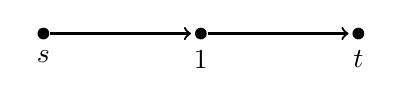
\begin{tikzpicture}[shorten >=1pt, thick]%[shorten >=1pt,node distance=2cm,>=stealth',thick]
  \node [shape=circle,fill=black,inner sep=1.5pt,label=below:$s$] (q0) at (0,0) {};
  \node [shape=circle,fill=black,inner sep=1.5pt,label=below:$1$] (q1) at (2,0) {};
  \node [shape=circle,fill=black,inner sep=1.5pt,label=below:$t$] (q2) at (4,0) {};
  \path[->] (q0) edge (q1) (q1) edge (q2);
\end{tikzpicture}
\end{center}
\caption[@descripcionCorta]{@descripcionLarga}
\label{grafo}
\end{figure}

\begin{enumerate}
\item 1
\item 2
\item 3
\end{enumerate}

\begin{tabular}{ll}
1 & 2\\ \hline
1 & 2\\
1 & 2\\
\end{tabular}

\blindtext. Tabla \ref{tabla:resultados}.

\begin{figure}[h]
\begin{alignat*}{1}
A\   & \longrightarrow B \mid C\\
\end{alignat*}
\caption[Gramática]{Gramática de un lenguaje.}
\label{gram}
\end{figure}

\blindtext
\begin{table}[h!]
\begin{center}
\begin{tabular}{llllll}
\multicolumn{4}{@{}c}{Nombre del experimento} \\
\midrule
              &    éxitos/intentos & tiempo (ms) & espacio (kB) \\
\midrule
instancia1          &        28/30 &    23 &       1.7 \\
instancia2          &        50/70 &    12 &       32.7 \\
\midrule
\end{tabular}
\end{center}
\caption[Resultados X/Y]{Resultados de X para Y}
\label{tabla:resultados}
\end{table}

\begin{equation}
\label{eq}
\Phi = (\forall x) (R x)
\end{equation}

En el Apéndice \ref{ad:A} se encuentra.

\chapter{Marco Tecnológico}
\label{ch:marco-tecnologico}
\lhead{Capítulo \getcurrentref{chapter}. \emph{\nameref{ch:marco-tecnologico}}}

\Blindtext

\chapter{Marco Metodológico}
\label{ch:marco-metodologico}
\lhead{Capítulo \getcurrentref{chapter}. \emph{\nameref{ch:marco-metodologico}}}

\Blindtext

\chapter{Desarrollo}
\label{ch:development}
\lhead{Capítulo \getcurrentref{chapter}. \emph{\nameref{ch:development}}}

{   % for \investigationfr, \designfr and \implementationfr to only exists here
\newenvironment{investigationfr}[1][]
    {\begin{coloredframe}[#1]{Investigación}{caribbeangreen}}
    {\end{coloredframe}}
\newenvironment{designfr}[1][]
    {\begin{coloredframe}[#1]{Diseño}{cerulean}}
    {\end{coloredframe}}
\newenvironment{implementationfr}[1][]
    {\begin{coloredframe}[#1]{Implementación}{crimson}}
    {\end{coloredframe}}

\begin{investigationfr}
\end{investigationfr}

\begin{designfr}
\end{designfr}

\begin{implementationfr}
\end{implementationfr}

\section{Ideas iniciales}

\begin{designfr}
Se comenzó con algunas ideas que consideramos básicas para el lenguaje.

\begin{itemize}
    \item El lenguaje debe ser explícito, es decir, no se deben inferir las ideas presentadas en un programa.
    \item La definición del lenguaje debe ser compacta.
    \item El lenguaje debe ser amistoso para principiantes.
    \item El sistema de tipos debe tener tipos dependientes.
    \item Los alcances del lenguaje deben ser determinados por la indentación.
\end{itemize}
\end{designfr}

\section{Expresiones, tipos y sus constructores}

\begin{designfr}
Ya que el lenguaje debe tener tipos dependientes, se decidió desde un principio que un tipo es sencillamente una expresión, no un elemento especial del lenguaje, hace que en cualquier parte donde se espera un tipo, debería poder escribirse cualquier expresión, mientras que el chequeo de tipos pase sin errores.

Al hacer estos dos elementos uno solo, se definieron las diferentes construcciones posibles de expresiones.

\begin{itemize}
    \item Aplicación de funciones
    \item Parentización
    \item Lambda funciones
    \item Pattern matching
    \item Alcance de declaraciones para una expresión (\inlinecode{where}, \inlinecode{let-in})
    \item Cuantificadores universales y existenciales de tipos
\end{itemize}
\end{designfr}

\section{Tipos y funciones, ¿abiertos o cerrados?}

\begin{designfr}
Nos preguntamos porqué se ha hecho una diferencia tan clara en otros lenguajes de programación funcionales entre lo que es una función, un tipo y un constructor de tipo, así que comenzamos con la idea de que todos éstos fueran declarados de la misma manera.

\begin{anglercode}
Bool : Type
True : Bool
False : Bool

not : Bool -> Bool
not True = False
not False = True
\end{anglercode}

Esta alternativa hacía que la única diferencia entre una función y un tipo es que no tenga declaraciones asociadas, pero el siguiente ejemplo nos dejó preguntándonos qué debería suceder:

\begin{anglercode}
Bool : Type
True : Bool
False : Bool

not : Bool -> Bool
not True = False
not False = True

True = False    -- ¿los pattern matching de `True` ahora son inválidos?
\end{anglercode}

¿Ahora \inlinecode{True} deja de ser algo sobre lo que se puede hacer pattern matching, como en la función \inlinecode{not}?; como podemos ver, da paso a que un programa deje de funcionar con tan solo una línea sospechosa.

Otro ejemplo que da paso a problemas sería agregar un constructor a un tipo que no se debe:

\begin{anglercode}
Bool : Type
True : Bool
False : Bool

not : Bool -> Bool
not True = False
not False = True

IDK : Bool

not IDK         -- ¿qué debería reportarse aquí?
\end{anglercode}

Aquí agregamos un nuevo constructor a el tipo \inlinecode{Bool} y aunque tenga sentido usarlo en la función \inlinecode{not}, pues espera algo del tipo \inlinecode{Bool}, el programa va a dar un error al correr, no al ser analizado por errores estáticos.

Así que decidimos introducir los tipos cerrados, éstos son tipos cuyos constructores son listados inmediatamente en un alcance nuevo, y no se le puede agregar más constructores.

\begin{anglercode}
Bool : Type where
    True : Bool
    False : Bool

not : Bool -> Bool
not True = False
not False = True
\end{anglercode}

Y ahora ninguna de las confusiones anteriores suedería, al declarar el \inlinecode{IDK} no habría problema, pero al llamar \inlinecode{not IDK}, el intepretador reportaría un error estático.

Luego vimos que \inlinecode{where} puede ser utilizado al final de cualquier expresión, por lo que no era un identificador que pudieramos utilizar para introducir los constructores, así que optamos por el identificador \inlinecode{with}. También el cambio muestra la diferencia semántica entre \inlinecode{where} y \inlinecode{with}, con el \inlinecode{where} se introduce un alcance sólo disponible en la expresión de éste, mientras que el \inlinecode{with} introduce elementos en el alcance exterior.

\begin{anglercode}
Bool : t where t = Type
    with
        True : Bool
        False : Bool
\end{anglercode}

Pero parecía interensante la idea de tipos que sus constructores pudieran ser agregados mientras se fueran necesitando, viene en mente un ejemplo de monedas del mundo con tan solo algunas monedas \textit{base}, para que el usuario agregue las de interés.

\begin{anglercode}
Currency : Type
USD : Nat -> Currency
EUR : Nat -> Currency

toUSD : Currency -> Currency
toUSD (USD n) = USD n
toUSD (EUR n) = USD (n * 1.1)

-- ...

XBT : Nat -> Currency   -- bitcoin
toUSD (XBT n) = USD (n * 400)
\end{anglercode}

Nos pareció lógico que si tenemos tipos abiertos y cerrados, deberíamos tener también funciones abiertas y cerradas; ya que estamos buscando enlazar lo más posible estos dos conceptos:

\begin{anglercode}
not : Bool -> Bool where
    not True = False
    not False = True
\end{anglercode}

Pero los tipos abiertos seguían sufriendo de los problemas presentados al principio, habría que hacer una diferencia más explícita entre tipos y funciones.

Los tipos, abiertos y cerrados, deben indicar explícitamente cuáles son sus constructores de tipos para evitar el problema antes mencionado, de forma que llegamos a la siguiente sintaxis:

\begin{anglercode}
closed Bool : Type with
    True : Bool
    False : Bool

not : Bool -> Bool
not True = False
not False = True

closed Nat : Type with
    Z : Nat             -- cero
    S : Nat -> Nat      -- sucesor

open Currency : Type with
    USD : Nat -> Currency
    EUR : Nat -> Currency

toUSD : Currency -> Currency
toUSD (USD n) = USD n
toUSD (EUR n) = USD (n * 1.1)

-- ...

reopen Currency with
    XBT : Nat -> Currency

toUSD (XBT n) = USD (n * 400)
\end{anglercode}

Además todo este análisis nos hizo darnos cuenta de que aunque los tipos, constructores de tipos y funciones compartan muchas cualidades, no son lo mismo, se diferencian semánticamente y ésto debería mostrarse en su definición también.

Haciendo finalmente claras las diferencias, dejamos de un lado la idea de funciones cerradas; aunque éstas pueden ser teóricamente interesantes, no conseguimos gran utilidad práctica, ya que de querer \textit{cerrar} una función abierta, simplemente se deben escribir todos los casos posibles de sus argumentos.

\begin{anglercode}
isUSD : Currency -> Bool
isUSD (USD _) = True
isUSD _ = False         -- *cierra* la función

-- ...

isUSD (XBT _) = True    -- este caso nunca correrá
\end{anglercode}
\end{designfr}

\section{Identificadores, ¿mayúsculas, minúsculas, ambas?}

\begin{designfr}
En un principio se consideró usar la convención de Haskell \cite{haskell}, que los constructores de tipos y tipos se escribieran con la primera letra mayúscula, y que los valores con la primera letra minúscula; de esta manera se podía distinguir sintácticamente entre ellos.

Pero esta idea tenía algunos problemas, por ejemplo, los identificadores que comenzaran con símbolos y no letras, ¿a qué clase pertenecerían?, además debemos recordar que con tipos dependientes, los tipos son expresiones como cualquier otra, por lo que una distinción sintáctica entre el \emph{uso} de tipos y valores no era conveniente. Finalmente decidimos que no habrá diferencia semántica entre identificadores que comiencen con mayúscula o minúscula.
\end{designfr}

\section{Identificadores inferidos}

\begin{designfr}
Como el lenguaje apunta a ser explícito, se evita la inferencia de tipos por completo, esto hace que no podamos tener varios identificadores iguales en un mismo alcance, ya que al usarlo no se sabe cuál usar; se podría inferir cuál identificador por el contexto en el que fue usado (e.g. \inlinecode{x:Nat} y \inlinecode{x:Bool}, en \inlinecode{not x} sólo funcionaría \inlinecode{x:Bool}), pero se opta por reportar un error.
\end{designfr}

\section{Cuantificadores: parámetros y argumentos implícitos}

\begin{designfr}
Como se busca un lenguaje explícito, todo identificador que se utilice en una expresión, debe estar previamente definido con un tipo acompañante, tomando inspiración de otros lenguajes con tipos dependientes llegamos a la idea de tener dos secciones de la firma de una función, la parte \emph{implícita}, que es el cuantificador universal; y la parte \emph{explícita}:

\begin{anglercode}
compose : { (a:Type) -> (b:Type) -> (c:Type) } -> (b -> c) -> (a -> b) -> a -> c
\end{anglercode}

Donde se escribe la parte implícita entre llaves (\inlinecode{\{} y \inlinecode{\}}) como un tipo más, y luego se escribe la parte explícita, donde todos los nombres introducidos en la parte implícita están disponibles. Esto nos dejaba con dudas acerca de cómo se podían escribir con una estructura similar los tipos existenciales.

Los argumentos implícitos se pasan a la función al comenzar su nombre con un caracter \emph{piso} (\inlinecode{\_}):

\begin{anglercode}
compose _Bool : { (b : Type) -> (c : Type) } -> (b -> c) -> (Bool -> b) -> Bool -> c
\end{anglercode}

Con esta sintaxis los parámetros implícitos son \emph{posicionales}, es decir, se pasan los argumentos con un orden específico. Esta manera de pasar argumentos implícitos nos da una restricción en los identificadores que se puedene escribir en el lenguaje, ya que ninguno podría comenzar con piso para poder diferenciarlos de argumentos implícitos.

Pero hay un mayor problema con la propuesta anterior, recordemos que en la teoría de tipos dependientes tenemos cuantificadores universales y existenciales; en un cuantificador universal no importa el orden de las variables declaradas, se puede especificar un valor para cualquera de las variables disponibles, es decir, los parámetros implícitos deberían ser todos accesibles para el pasaje de argumentos implícitos. Así llegamos a otra propuesta que separa completamente la sintaxis de firmas y de cuantificadores:

\begin{anglercode}
compose : { a:Type, b:Type, c:Type } (b -> c) -> (a -> b) -> a -> c
\end{anglercode}

Con esta nueva sintaxis podemos pasar argumentos implícitos en el orden que sea necesario:

\begin{anglercode}
compose { b = Nat, c = Bool } : { a:Type } (Nat -> Bool) -> (a -> Nat) -> a -> Bool
\end{anglercode}

Con esta nueva los parámetros implícitos son \emph{nombrados}, es decir, se pasan los argumentos en el orden que nos convenga, sin importar su posición, y los parámetros explícitos se mantienen posicionales.

Finalemente decidimos hacer un último cambio a esta sintaxis para hacer obvio que se trata de un cuantificador:

\begin{anglercode}
compose : forall a:Type, b:Type, c:Type . (b -> c) -> (a -> b) -> a -> c
\end{anglercode}

Ahora la definición se asemeja mucho más a un cuantificador, haciendo más explícito su uso, y además podemos acceder a todas las variables declaradas y especificarlas.

Se consideró usar la palabra \inlinecode{product} en vez de \inlinecode{forall}, pero se decidió ir por una referencia directa a lógica simbólica, aunque estos se consideren los tipos producto.

De igual forma, se definen los tipos existenciales con la palabra \inlinecode{exists}, aunque se consideró la palabra \inlinecode{sum}:

\begin{anglercode}
vfilter : forall t:Type, n:Nat . (t -> Bool) -> Vect n t -> exists m:Nat . Vect m t
\end{anglercode}

Logrando una estructura parecida entre los cuantificadores universales y existenciales. El cuantificador existencial \emph{no} puede recibir argumentos implícitos. Esta sintaxis es \emph{azúcar sintáctica} para los cuantificadores existenciales, ya que estos están definidos en el lenguaje.
\end{designfr}

\section{El \emph{cuantificador} de selección}

\begin{designfr}
Nos dimos cuenta de que podemos querer introducir nombres para parámetros explícitos, es decir, lo que normalmente haríamos con un cuantificador universal, pero en vez de ser \emph{para todo} que sea para el valor dado. Esta idea se maneja en los lenguajes estudiados colocando una asociación de nombre directamente:

\begin{anglercode}
id' : (t : Type) -> t -> t
id' t x = x
\end{anglercode}

Se entiende, pero nos pareció poco intuitivo, así que preferimos agregarle la palabra \inlinecode{select} para hacer obvio que se acerca al funcionamiento de los cuantificadores.

\begin{anglercode}
id' : (select t : Type) -> t -> t
id' t x = x
\end{anglercode}

Además se lee \emph{\enquote{selecciona un \inlinecode{Type}, que llamaremos \inlinecode{t}}}.
\end{designfr}

\section{¿Identificador o caracter?}

\begin{designfr}
Los caracteres literales suelen escribirse usando comillas simples (\inlinecode{'}), así que se decidió que ningún identificador puede empezar con una comilla simple, ya que se estaría esperando un caracter literal. Comilla simple es el único \emph{símbolo} que está en ambas categorías de identificadores, la de símbolos y la de letras.

\begin{anglercode}
'a'     -- caracter
a''     -- identificador
+''     -- identificador
\end{anglercode}
\end{designfr}


\section{Identificadores, evitando confusiones}

\begin{designfr}
Desde un principio se aceptó la idea de poder usar símbolos en los identificadores como \inlinecode{+}, \inlinecode{*} y demás, pero para facilitar el uso del lenguaje, se decidió que tendríamos dos categorías de caracteres, una para símbolos y otra para letras. De manera que ciertos caracteres, a pesar de estar juntos, se tomarían como identificadores separados:

\begin{anglercode}
var         -- var
v0          -- v0
0v0         -- 0 v0
++          -- ++
var++v0     -- var ++ v0
\end{anglercode}
\end{designfr}

\section{No me importa; es más, te lo digo en inglés, I \emph{don't care}}

\begin{designfr}
En una función puede haber casos en que un argumento no es importante para su valor resultante, a estos argumentos se les puede asignar un nombre que no usaremos, o indicar explícitamente que no es importante con algún identificador, a éste se le suele llamar \emph{don't care}.

\begin{anglercode}[alsoletter={?},morekeywords={?}]
const : forall t:Type, v:Type . t -> v -> t
const x ? = x
\end{anglercode}

Donde el caracter \inlinecode{?} indica que no importa ese valor, luego se decidió cambiar este caracter a \inlinecode{\_}, ya que el signo de interrogación puede transmitir la idea de que \emph{no sabemos} qué será el argumento, cuando lo que se quiere transmitir es que \emph{no importa}. Se eligió \inlinecode{\_} porque es el caracter típicamente usado por otros lenguajes para lo miso, y visualmente, al llamar tan poco la atención transmite su poca importancia.

\begin{anglercode}[morekeywords={\_}]
const : forall t:Type, v:Type . t -> v -> t
const x _ = x
\end{anglercode}
\end{designfr}

\section{Operadores ahuecados}

\begin{designfr}
Un lenguaje didáctico sin operadores puede hacer curva de aprendizaje muy \emph{empinada}, por lo que la posibilidad de definir operadores es escencial. Se propuso usar \emph{operadores mixfijos}, estos funcionan para definir las \emph{partes} de un operador y sus \emph{huecos}, que es donde irían sus operandos; para indicar los huecos de un operador, usaremos el caracter piso (\inlinecode{\_}).

\begin{anglercode}
if_then_else_ : forall t:Type . Bool -> t -> t -> t
if True  then x else _ = x
if False then _ else y = y
\end{anglercode}

Esto nos crea una restricción sobre los identificadores, estos no pueden contener dos \inlinecode{\_} seguidos, ya que no sabríamos dónde termina un argumento y comienza el siguiente.

Un identificador con \inlinecode{\_} puede usarse como operador, colocando los argumentos en los huecos, o como una función normal escribiendo el identificador con los \inlinecode{\_} incluidos.

\begin{anglercode}
if_then_else_ : forall t:Type . Bool -> t -> t -> t
if_then_else_ True  x _ = x
if_then_else_ False _ y = y
\end{anglercode}

Nótese que se usa \inlinecode{\_} tanto para \emph{don't care} como para los huecos de los identificadores, e.g. \inlinecode{if\_then\_else\_\ False\ \_\ y}.
\end{designfr}

\section{Huecos entre identificadores}

\begin{designfr}
Gracias a la nueva sintaxis para operadores, se decidió que un las partes distintas de un identificador podrían ser de distintas categorías, es decir, pudiendo mezclarlas sólo cuando hay un \inlinecode{\_} de por medio.

\begin{anglercode}
if_??_:_ : forall t:Type . Bool -> t -> t -> t
if True  ?? x : _ = x
if False ?? _ : y = y
\end{anglercode}
\end{designfr}

\section{Definición de operadores}

\begin{designfr}
En un principio se consideró que si un identificador tiene \inlinecode{\_} se consideraría automáticamente un operador y tendría una precedencia y asociatividad por defecto, pero decidimos abandonar esa idea, pues podría generar comportamientos inesperados por usuarios. Así que llegamos a una definición para estos, donde no importa si el identificador es de una función o no, o está definido o no. Lo que se expresa es una regla de \emph{reordenamiento} de identificadores.

\begin{anglercode}[label=lst:operatorsdefinition]
operator |_|                closed
operator if_then_else_      prefix  0
operator _==_               infixN  2
operator _+_                infixL  4
operator _-_                infixL  4
operator _*_                infixL  5
operator _/_                infixL  5
operator _^_                infixR  6
operator -_                 prefix  7
operator _!                 postfix 8

-- ...

if | a * b + c - d | == e then f ! else - f
-- if_then_else_ (_==_ (|_| (_-_ (_+_ (_*_ a b) c) d)) e) (_! f) (-_ f)
\end{anglercode}
\end{designfr}

\section{Módulos: importación}

\begin{designfr}
Los módulos son una gran ayuda para la organización de código, permite seprar un conjunto de funciones relacionadas independiente de otro.

Para la importación se coloca la opción de hacer importar los nombres de manera cualificada, esto es, anexando un identificador a todos los identificadores importados de un módulo:

\begin{anglercode}
import Nat as N         -- N.Nat, N.Z, N.S, N._+_, N.even, N.odd, ...
\end{anglercode}

También se debe poder limitar la lista de cosas a importar:

\begin{anglercode}
import Nat (Nat, Z, S, _+_, odd)
\end{anglercode}

Pero una duda que nos dejó pensativos es si importar un módulo también introduce sus operadores en el módulo actual, nos pareció que esto debía hacerce de manera explícita, pues puede generar comportamientos inesperados si no:

\begin{anglercode}
import Nat (Nat, Z, S, _+_, odd, operator _+_)
\end{anglercode}

Y esto nos puso a pensar que sería interesante hacer lo que se importa más explícito aún, que con tan solo ver esa línea puedes saber más o menos de qué se trata, sin tener que revisar el módulo en cuestión. Así que se debe indicar qué tipo de elemento se está importando también:

\begin{anglercode}
-- N.Nat, N.Z, N.S, N._+_, N.Command
import Nat (closed Nat(Z, S), _+_, operator _+_, open Command) as N

reopen N.Command with
    Jump : N.Nat -> N.Command
\end{anglercode}
\end{designfr}

\section{Módulos: exportación}

\begin{designfr}
La exportación debía entonces seguir la misma idea en su de identificadores. Se asume que si no se declara una línea de exportación, se exportan todos los contenidos del módulo.

\begin{anglercode}[morekeywords={export}]
export (closed Nat(Z, S), _+_, operator _+_, open Command(Print))

closed Nat : Type with
    Z : Nat
    S : Nat -> Nat

operator _+_ infixL 4
_+_ : Nat -> Nat -> Nat
Z + n = n
S m + n = S (m + n)

open Command : Type with
    Print : String -> Command
\end{anglercode}

El único problema con esta sintaxis de exportación es que no sabemos cómo se llama el archivo con ver el código, que es importante porque se importan módulos con el nombre del archivo. Se agregó el nombre del módulo:

\begin{anglercode}
module Nat exports (closed Nat(Z, S), _+_, operator _+_, open Command(Print))
\end{anglercode}

En caso de querer exportar el módulo completo, se debe iniciar igual con el nómbre del módulo (e.g. \inlinecode{module Nat}).
\end{designfr}

\section{Escribiendo un \emph{lexer} con inspiración}

\begin{designfr}
El analizador léxico (\emph{lexer}) de nuestro lenguaje no sería el típico caso de separar tokens e ignorar comentarios, tenemos que obtener la información de alcances dependiendo de la indentación, caracteres literales, cadenas de caracteres, números literales e incluimos anidación de comentarios. Los tabuladores (\emph{tabs}) son equivalentes a cuatro (4) espacios.
\end{designfr}

\begin{investigationfr}
Para lograr esto, nos fijamos en lenguajes que también usen indentación para definir alcances, conseguimos un analizador sintáctico de Python escrito en Haskell \cite{python-parser} que ayudó con algunas nociones de cómo lograr esto, pero el analizador léxico de GHC \cite{ghc} fue la mayor influencia para la escritura del analizador léxico.
\end{investigationfr}

\begin{implementationfr}
Utilizamos la herramienta \emph{Alex} \cite{alex} para la generación del analizador léxico.

Se listan identificadores reservados para que reconozca el analizador léxico y se especifica algunos que introducen un nuevo alcance, éstos \emph{esperan} una indentación mayor a la usada anteriormente y de ahí en adelante se considera el mismo alcance todo lo que esté en la indentación recién definida. Los identificadores que introducen un nuevo alcance son \inlinecode{where}, \inlinecode{let}, \inlinecode{with} y \inlinecode{of}.

Se reportan errores por caracteres literales inválidos y comentarios de bloque que no fueron cerrados. También se generan advertencias cuando el código contiene tabuladores (\emph{tabs}), pues pueden considerarse una mala práctica cuando la indentación afecta un programa.

Los comentarios anidados se llevarón a cabo manteniendo una pila de estados del analizador léxico, donde al conseguir un \inlinecode{\{-}, sin importar qué estado esté en el tope la pila, se empila un estado indicando que está en un comentario, y al conseguir un \inlinecode{-\}} con un estado de comentario en el tope, se desempila éste.

Tomamos de GHC la idea de que una línea con indentación mayor a la anterior indica que se debe tomar como la misma línea. Un ejemplo donde se refleja el funcionamiento; no es código válido para el lenguaje:

\begin{anglercode}[deletekeywords={as}]
top1 where
        scope1
        scope2
            same line as scope2
    same line as top1
top2 where
    scope3
top3
    same line as top3

{-
    {-
        {^ y ^} indican un alcance
        ^;      indica una línea nueva
        <eof>   indica el final del archivo
    -}

    La salida del analizador léxico:
    {^
        top1 where {^
            scope1 ^;
            scope2 same line as scope2
        ^} same line as top1 ^;
        top2 where {^
            scope3
        ^} ^;
        top3 same line as top3
    ^} <eof>
-}
\end{anglercode}
\end{implementationfr}

\section{Escribiendo el \emph{parser}}

\begin{implementationfr}
Utilizamos la herramienta \emph{Happy} \cite{happy} para la generación del analizador sintáctico. Es la etapa que sigue al análisis léxico. Se reportan errores considerados \emph{comunes} con una explicación, los que no se consideraron simplemente reportan un error de \emph{parseo}.

{   % for the commands to only exist here
\renewcommand{\emph}[1]{\textbf{\textit{#1}}}
\renewcommand{\_}{\:\:}

\newcommand{\maybe}[1]{\left[ \_ #1 \_ \right]}
\newcommand{\listZ}[1]{#1^{*}}
\renewcommand{\list}[1]{#1^{+}}
\newcommand{\listSepZ}[2]{#1^{* [ \_ #2 \_ ]}}
\newcommand{\listSep}[2]{#1^{+ [ \_ #2 \_ ]}}

% literal
\newcommand{\lt}[1]{\textbf{\color{darkcandyapplered}\text{#1}}}

\newcommand{\scope}[1]{\widehat{\{} \_ #1 \_ \widehat{\}}}
\newcommand{\parens}[1]{\lt{(} \_ #1 \_ \lt{)}}
\newcommand{\scolon}{\widehat{;}}

\allowdisplaybreaks
\footnotesize
\begin{align*}
\maybe{\emph{p}} ::=& \_ \lambda \_ | \_ \emph{p}
\\
\list{\emph{p}} ::=& \_ \emph{p} \_ | \_ \emph{p}^{+} \_ \emph{p}
\\
\listZ{\emph{p}} ::=& \_ \lambda \_ | \_ \emph{p}^{+}
\\
\listSep{\emph{p}}{\emph{sep}} ::=
    & \_ \emph{p} \_
    | \_ \listSep{\emph{p}}{\emph{sep}} \_ \emph{sep} \_ \emph{p}
\\
\listSepZ{\emph{p}}{\emph{sep}} ::=
    & \_ \lambda \_
    | \_ \listSep{\emph{p}}{\emph{sep}}
\\
\\
Module ::=& \_ \scope{Top \_ Body}
\\
\\
Top ::=& \_ \lt{module} \_ Id \_ \maybe{Export} \_ \listZ{Import}
\\
Export ::=& \_ \lt{exports} \_ \parens{\listSepZ{Id}{\lt{,}}}
\\
Import ::=& \_ \lt{import} \_ Id \_ \maybe{as \_ Id} \_
    \maybe{\parens{\listSepZ{Id}{\lt{,}}}}
\\
\\
Body ::=& \_ \list{Stmt}
\\
Stmt ::=
     & \_ TypeBind
\\
    |& \_ FuncDef
\\
    |& \_ \lt{open} \_ TypeBind \_
        \maybe{ \lt{with} \_ \scope{\list{TypeBind}} }
\\
    |& \_ \lt{reopen} \_ Id \_  \lt{with} \_
        \scope{\list{TypeBind}}
\\
    |& \_ \lt{closed} \_ TypeBind \_  \lt{with} \_
        \scope{\list{TypeBind}}
\\
    |& \_ \lt{operator} \_ Id \_ \lt{prefix}  \_ Nat
\\
    |& \_ \lt{operator} \_ Id \_ \lt{postfix} \_ Nat
\\
    |& \_ \lt{operator} \_ Id \_ \lt{infixL}  \_ Nat
\\
    |& \_ \lt{operator} \_ Id \_ \lt{infixR}  \_ Nat
\\
    |& \_ \lt{operator} \_ Id \_ \lt{infixN}  \_ Nat
\\
    |& \_ \lt{operator} \_ Id \_ \lt{closed}
\\
%     |& \_ \lt{open} \_ \lt{scope} \_ Id \_
%         \maybe{\lt{with} \_ \list{BehaviourDef}}
% \\
%     |& \_ \lt{reopen} \_ \lt{scope} \_ Id \_ \lt{with} \_ \list{BehaviourDef}
% \\
%     |& \_ \lt{closed} \_ \lt{scope} \_ Id \_ \lt{with} \_ \list{BehaviourDef}
% \\
%     |& \_ \lt{behaviour} \_ Id \_ \lt{on} \_ TypeBind \_ \lt{defines} \_
%         \scope{\list{TypeBind}}
% \\
%      & \_\_\_\_ \maybe{\lt{with} \_ \scope{\list{FuncDef}}}
% \\
%     |& \_ BehaviourDef
% \\
\\
TypeBind ::=& \_ Id \_ \lt{:} \_ Expr
\\
FuncDef ::=& \_ \list{Argument} \_ \lt{=} \_ Expr
\\
% BehaviourDef ::= & \_ Id \_ \lt{is} \_ Id \_ \lt{with} \_ \scope{\list{FuncDef}}
% \\
Argument ::=
    & \_ \lt{\textunderscore} \_ | \_ Id \_ | \_ \parens{\list{Argument}}
\\
\\
Expr ::=& \_ Expr' \_ \maybe{\lt{where} \_ Body}
\\
Expr' ::=
%      & \_ \lt{\textbackslash} \_ \list{Argument} \_ \lt{:} \_ Expr \_
%         \lt{=} \_ Expr'
% \\
    |& \_ \lt{let} \_ \scope{Body} \_ \lt{in} \_ Expr'
\\
    |& \_ \lt{forall} \_ \listSep{TypeBind}{\lt{,}} \_ \lt{.} \_ Expr'
\\
    |& \_ \lt{exists} \_ TypeBind \_ \lt{.} \_ Expr'
\\
    |& \_ \lt{select} \_ TypeBind
\\
    |& \_ \lt{case} \_ Expr' \_ \lt{:} \_ Expr \_ \lt{of} \_
        \scope{\list{FuncDef}}
\\
    |& \_ Term \_ Expr'
\\
    |& \_ Term
\\
Term ::=
    & \_ Id \_ | \_ Literal \_ | \_ \parens{Expr} \_
    | \_ \lt{\{} \_ \listSep{(Id \_ \lt{=} \_ Expr)}{\lt{,}} \_ \lt{\}}
\\
Literal ::=& \_ Nat \_ | \_ Char \_ | \_ String
\\
Nat ::=& \_ \left<natural \_ number \_ literal\right>
\\
Char ::=& \_ \left<character \_ literal\right>
\\
String ::=& \_ \left<string \_ literal\right>
\\
Id ::=& \_ \left<identifier\right>
\end{align*}
\captionof{figure}{Gramática final del analizador sintáctico}
\label{fig:parser-grammar}
}

Esta gramática presenta una construcción de expresión \inlinecode{case-of} del lenguaje que aún no han sido explicada en este capítulo, pero se incluye por completitud. Ésta será explicada en la sección \ref{case-of}.

\end{implementationfr}

\section{Operadores \emph{mixfijos} en acción}

\begin{investigationfr}
La idea de usar operadores mixfijos surgió del lenguaje de programación \emph{Agda} \cite{agda}, así que nos apoyamos en la investigación que se hizo para la implementación de estos en ese lenguaje para nuestra propia implementación. \textcite{parsing-mixfix-operators} proponen una gramática a ser derivada directamente de los operadores, asociatividades y precedencias declaradas; los pasos a seguir son (1) construir un grafo dirigido acíclico de precedencia donde un arco del nodo \inlinemath{p} al nodo \inlinemath{q}, (\inlinemath{p \longrightarrow q}) representa que los operadores en el nodo \inlinemath{q} tienen mayor precedencia que los operadores en el nodo \inlinemath{p}; (2) crear una gramática \emph{posiblemente} ambigua basada en la información del grafo. Si se utiliza la gramática presentada en el artículo con las modificaciones que proponen en los operadores definidos en \ref{lst:operatorsdefinition} se obtiene el siguiente grafo:

\begin{center}
\includegraphics[width=0.75\textwidth]{operator-graph.pdf}
\captionof{figure}{Grafo de precedencia de operadores}
\label{fig:operator-graph}
\end{center}

Como podemos ver, se obtiene un grafo de precedencia lineal, ya que en nuestro lenguaje no se puede definir explícitamente la precedencia entre dos operadores, sino que se asigna un \emph{nivel de precedencia}. Por lo que podemos reducir la idea de un grafo de precedencia a una lista de precedencias, donde un valor de precedencia mayor indica una mayor precedencia (\emph{¡duh!}); los operadores con asociatividad cerrada (\inlinecode{closed}) se consideran como la menor precedencia.

{   % for \overp and \_ to only exist here
\newcommand{\overp}[1]{\overset{#1}{p}}
\renewcommand{\emph}[1]{\textbf{\textit{#1}}}
\renewcommand{\_}{\:\:}

\allowdisplaybreaks
\footnotesize
\begin{align*}
expr ::=
    & \left( \bigvee \_ \hat{p} \_ \cdotp \_
        \text{$p$ es un nivel de precedencia} \right) \_
    | \_ closed^{+}
\\
\hat{p} ::=
     & \_ \overp{\uparrow} \_ op_p^{infixN} \_ \overp{\uparrow} \\
    |& \_ \overp{\rightarrow}^{+} \_ \overp{\uparrow} \\
    |& \_ \overp{\uparrow}\quad \overp{\leftarrow}^{+}
\\
\overp{\rightarrow} ::=
    & \_ op_p^{prefix} \_
    | \_ \overp{\uparrow} \_ op_p^{infixR}
\\
\overp{\leftarrow} ::=
    & \_ op_p^{postfix} \_
    | \_ \overp{\uparrow} \_ op_p^{infixL}
\\
\overp{\uparrow} ::=
    & \left( \bigvee \hat{q} \_ \cdotp \_ p \_ < \_ q \right) \_
    | \_ closed^{+}
\\
closed ::=
    & \left<identificador\right> \_
    | \_ \boldsymbol{(} expr \boldsymbol{)} \_
    | \left( \bigvee \_ op_p^{closed} \right)
\\
op_p^{\emph{asoc}} ::=
    & \left( \bigvee n_1\ expr\ n_2\ expr\ \cdots\ n_k \_ \cdotp \_
        \parbox{0.3\textwidth}{\footnotesize$n_1,\ldots,n_k$ son las partes de un operador en el nivel $p$ con la asociatividad $asoc$} \right)
\\
\emph{p}^{+} ::=
    & \_ \emph{p} \_
    | \_ \emph{p}^{+} \_ \emph{p} \_
\end{align*}
\captionof{figure}{Gramática de precedencia de operadores basada en \cite{parsing-mixfix-operators}}
\label{fig:mixfix-grammar}
}
\end{investigationfr}

\begin{implementationfr}
En nuestra implementación del analizador sintáctico de operadores mixfijos, no construímos un grafo sino una \emph{lista de niveles de precedencia}, ya que la precedencia entre operadores no es asignada entre dos operadores únicamente, sino que se asigna un valor para comparación con todos los otros operadores presentes.

Utilizamos \emph{Megaparsec}, una librería de \emph{combinadores de analizador sintácticos} \cite{megaparsec}, y a partir de la lista de precedencias y la gramática \ref{fig:mixfix-grammar}, se genera un analizador sintáctico que \emph{reorganiza las expresiones en una lista de expresiones} y las analiza recursivamente. En un princpio el analizador sintáctico resultante podía ser muy lento si habían muchas definiciones de operadores en el programa, así que se hace un análisis previo del nivel de la lista de expresiones para incluir únicamente operadores que \emph{alguna de sus partes} esté en ésta, y se analiza antes de cada nivel para incluir los operadores adecuados por separado; logrando así unos resultados de tiempo aceptables.
\end{implementationfr}

\section{Clases de tipos, tipos y constructores azucarados}

\begin{investigationfr}
\textcite{less-ad-hoc-polymorphism} presentan las \emph{clases de tipos}, una herramienta para manejar el poliformismo de manera más organizada, es decir, poder utilizar un mismo identificador de función para diferentes tipos. Aquí se presenta un ejemplo en Haskell.

\begin{haskellcode}
-- tiene un `forall t:Type .` implícito
class Eq t where
    (==) :: t -> t -> Bool
    (/=) :: t -> t -> Bool

    x /= y = not (x == y)
    x == y = not (x /= y)

-- tiene un `forall t:Type .` implícito
instance Eq Bool where
    True == True = True
    False == False = True
    _ == _ = False

elem :: Eq t => t -> [t] -> True
elem _ [] = False
elem x (y:ys) = x == y || elem x ys

elem False [False, True]    -- True
\end{haskellcode}

En un primer momento no se consideraron necesarias para nuestro lenguaje, aunque su facilidad de uso es innegable, porque creíamos que se podía lograr el mismo comportamiento usando tipos dependientes.

\begin{anglercode}
closed Eq : Type -> Type with
    EqI : forall t:Type . (t -> t -> Bool) -> Eq t

-- las funciones que define la *clase*
equal : forall t:Type . Eq t -> t -> t -> Bool
equal (EqI eq) = eq
unequal : forall t:Type . Eq t -> t -> t -> Bool
unequal (EqI eq) = not eq

BoolEq : Eq Bool
BoolEq = EqI op
    where
        op : Bool -> Bool -> Bool
        op True  True  = True
        op False False = True
        op _     _     = False

elem : forall t:Type . Eq t -> t -> List t -> t
elem _         _ Nil = False
elem tEq x (y :: ys) = (equal tEq) x y || elem (EqI op) x ys

elem BoolEq False (False :: True :: Nil)    -- True
\end{anglercode}

La mayor diferencia es que para utilizar estas funciones en nuestro lenguaje, se debe pasar la \emph{instancia} a utilizar explícitamente. De hecho, esta es una manera válida para plantear las clases de tipos \cite{scrap-type-classes}, como azúcar sintáctica para tipos y constructores.
\end{investigationfr}

\section{Comportamientos, o: cómo aprendí a usar \emph{clases de tipos} y a amar el polimorfismo}

\begin{designfr}
Decidimos plantear una posible sintaxis para las clases de tipos. En los lenguajes estudiados se les suele llamar \enquote{clase} (\inlinecode{class}); pero nos pareció más intuitivo llamarlas \enquote{comportamientos} (\inlinecode{behaviour}), pues es una definición de que un tipo se \emph{comporta} de cierta forma.

\begin{anglercode}
behaviour Eq on t : Type defines
    _==_ : t -> t -> Bool
    _/=_ : t -> t -> Bool
  with
    a /= b = not (a == b)
    a == b = not (a /= b)

Bool is Eq with
    True  == True  = True
    False == False = True
    _     == _     = False

elem : forall t:Type is Eq . t -> List t -> Bool
elem _ Nil = False
elem x (y :: ys) = x == y || elem x ys
\end{anglercode}

Se cambiaron algunos identificadores reservados, pero la definición e instanciación es equivalente a la de clases de tipos vista en otros lenguajes. Una diferencia considerable es la del requerimiento de clases, e.g. \inlinecode{Type is Eq}, ya que se pierde la traducción intuitiva con la solución de azúcar sintáctica de tipos y constructores presente en los lenguajes estudiados.
\end{designfr}

\section{Comportamientos múltiples}

\begin{designfr}
El uso de comportamientos puede facilitar mucho el uso de polimorfismo, pues no hay que pasar explícitamente las instancias a utilizar.

Un problema que presentan es para los tipos que poseen más de una posible instancia de un comportamiento:

\begin{anglercode}
behaviour Semigroup on t:Type defines
    _<+>_ : t -> t -> t
behaviour Monoid on t : Type is Semigroup defines
    neutral : t

Nat is Semigroup with
    _<+>_ = _+_

Nat is Semigroup with
    _<+>_ = _*_
\end{anglercode}

Para solucionar este problema conseguimos dos propuestas que ninguna nos pareció muy satisfacotira, la primera es \emph{envolver} el tipo en un constructor específicamente para la instancia.

\begin{anglercode}
closed Sum : Type with
    NatSum : Nat -> Sum
Sum is Semigroup with
    NatSum a <+> NatSum b = NatSum (a + b)

closed Product : Type with
    NatProduct : Nat -> Product
Product is Semigroup with
    NatProduct a <+> NatProduct b = NatProduct (a * b)
\end{anglercode}

La segunda opción es \emph{instancias nombradas}, de manera que para utilizar la instancia habría que colocar su identificador para indicar la que se quiere utilizar. De esta segunda opción surgió otra propuesta, hacer \emph{alcances de instancias nombrados}, es decir, alcances donde se agrupan instancias relacionadas.

\begin{anglercode}
scope Sum with
    Nat is Semigroup with
        _<+>_ = _+_
    Nat is Monoid with
        neutral = Z

scope Product with
    Nat is Semigroup with
        _<+>_ = _*_
    Nat is Monoid with
        neutral = S Z
\end{anglercode}

Igual se podrían hacer instancias en el alcance global, pero se usa cuando se necesita una instancia especial aparte de la principal, (e.g. instancias de \inlinecode{Show} en un alcance \inlinecode{AST}, para mostrar un árbol de sintaxis abstracta), o cuando hay más de una instancia válida.

Este problema no existe si usamos tipos y constructores, ya que toda \emph{instancia} debe ser nombrada.

\begin{anglercode}
closed Semigroup : Type -> Type with
    SemigroupI : forall t:Type . (t -> t -> t) -> Semigroup t

append : forall t:Type . Semigroup t -> (t -> t -> t)
append (SemigroupI op) = op

closed Monoid : Type -> Type with
    MonoidI : forall t:Type . (t -> t -> t) -> t -> Monoid t

-- obtener una instancia de Monoid por una de Semigroup (*superclass*)
Monoid'Semigroup : forall t:Type . Semigroup t -> t -> Monoid t
Monoid'Semigroup (SemigroupI op) e = MonoidI op e

mappend : forall t:Type . Monoid t -> (t -> t -> t)
mappend (MonoidI op _) = op

mempty : forall t:Type . Monoid t -> t
mempty (MonoidI _ e) = e

SumSemigroup : Semigroup Nat
SumSemigroup = SemigroupI _+_
SumMonoid : Monoid Nat
SumMonoid = Monoid'Semigroup SumSemigroup Z

ProductSemigroup : Semigroup Nat
ProductSemigroup = SemigroupI _*_
ProductMonoid : Monoid Nat
ProductMonoid = Monoid'Semigroup ProductSemigroup (S Z)
\end{anglercode}
\end{designfr}

\section{Comportamientos, ¿valen la pena?}

\begin{designfr}
Quedamos dudosos acerca de la necesidad de comportamientos, tenemos varias razones a favor:

\begin{itemize}
    \item Introducen identificadores automáticamente para su uso (e.g. \inlinecode{neutral}).
    \item Facilitan la representación de \emph{pilas de comportamientos}, es decir, la necesidad de uno para la definición de otro.
    \item Permiten escribir código mucho más breve y ordenado.
    \item \#TODO.
\end{itemize}

También tenemos razones a favor de solamente usar tipos y constructores:

\begin{itemize}
    \item Permiten expresar código explícito sobre cuál \emph{instancia} se utilizará en cada aplicación funcional.
    \item Permiten simular comportamientos de múltipes parámetros.
    \item \#TODO.
\end{itemize}

Por lo que decidimos que no deben formar parte del diseño principal del lenguaje, pero que en caso de incluirlos en una implementación, se debe usar la sintaxis propuesta.
\end{designfr}

\section{Lamda funciones explícitas}

\begin{designfr}
Las lambda funciones son una de las construcciones clásicas de los lenguajes de programación funcional, nos parecía obvio que debían estar en el diseño, pero suelen ser presentadas en los lenguajes estudiados sin asociación de tipos a los argumentos ni a su tipo; como buscamos un lenguaje explícito, esto iba en contra de la filosofía que presenta el lenguaje en el resto del diseño.

\begin{anglercode}
\ x y => x :: y :: Nil      -- ¿de qué tipo es la función?
\end{anglercode}

Así que propusimos diversas sintaxis para usar en el lenguaje:

\begin{anglercode}
-- anotación de tipos por argumento y salida
\ (x : Nat) (y : Nat) : List Nat => x :: y :: Nil

-- anotación de tipo de la función completa
\ x y : Nat -> Nat -> List Nat => x :: y :: Nil
\end{anglercode}

Pero ninguna nos convenció, así que decidimos que las lambdas funciones tampoco deben formar parte del diseño principal del lenguaje, pero que en caso de incluirlas en un implementación, se debe usar la sintaxis de \emph{anotación de tipo de la función completa}.
\end{designfr}

\section{Deconstrucción de expresiones con pattern matching y análisis por caso}
\label{case-of}

\begin{designfr}
Ya habiendo avanzado bastante en la implementación nos dimos cuenta de que no había cómo deconstruir una expresión para evaluar sus casos, se nos ocurrió colocar los pattern matching en un \inlinecode{where}, pero se veían muy parecidos a una definición de función, necesitamos una sintaxis que muestre la diferencia de semántica. De manera que surgieron las siguientes tres opciones:

\begin{anglercode}[morekeywords={pattern}]
-- inspirado en Idris
evenNlength : forall t:Type . List t -> Tuple Bool Nat
evenNlength Nil = (True; Z)
evenNlength (x :: xs)
    with evenNlength xs
        | (ev; ln) = (not ev; S ln)

-- en `where` pero con un identificador reservado `pattern`
evenNlength : forall t:Type . List t -> Tuple Bool Nat
evenNlength Nil = (True; Z)
evenNlength (x :: xs) = (not ev; S ln)
    where
        pattern (ev; ln) = evenNlength xs

-- case-of como en Haskell
evenNlength : forall t:Type . List t -> Tuple Bool Nat
evenNlength Nil = (True; Z)
evenNlength (x :: xs) =
    case evenNlength xs of
        (ev; ln) = (not ev; S ln)
\end{anglercode}

La opción del \inlinecode{where} fue descartada pues no se pueden representar distintos casos para un patrón, la opción del \inlinecode{with} fue descartada porque sólo funcionaría al principio de una definición de función, dejando como la única opción viable la de \inlinecode{case-of}. Ninguna de estas opciones asocia la expresión a evaluar con su tipo explícitamente, así que modificamos la sintaxis del \inlinecode{case-of}, agergando el tipo de la expresión:

\begin{anglercode}
evenNlength : forall t:Type . List t -> Tuple Bool Nat
evenNlength Nil = (True; Z)
evenNlength (x :: xs) =
    case evenNlength xs : Tuple Bool Nat of
        (True ; ln) = (False; S ln)
        (False; ln) = (True ; S ln)
\end{anglercode}
\end{designfr}

}

\chapter{Resultados}
\label{ch:results}
\lhead{Capítulo \getcurrentref{chapter}. \emph{\nameref{ch:results}}}


\chapter{Conclusiones y Recomendaciones}
\label{ch:conclusions}
\lhead{\emph{\nameref{ch:conclusions}}}

\Blindtext

% Incluir recomendaciones para trabajos futuros
\blindenumerate


% El estilo de la bibliografía es AAAI, definido en el archivo aaai.bst.
\label{bibliography}
\printbibliography
\lhead{\emph{Bibliografía}}
\addtocontents{toc}{\vspace{2em}}
\addcontentsline{toc}{chapter}{Bibliografía}

% Apéndices
\appendix
\chapter{@nombreApendice}
\label{ad:A}
\lhead{Apéndice A. \emph{\nameref{ad:A}}}

% En los apéndices se incluye cualquier información que no sea esencial para la
% comprensión básica del trabajo, pero provea ejemplos y casos de estudio
% extendidos que permitan un análisis más exhaustivo.

\section{@sección}
\blindtext

\subsection{@subsección}
\Blindtext

``Saludo''.

\begin{figure}[h!]
\centering
\includegraphics[width=0.5\textwidth]{operator-graph.pdf}
\caption[Grafo]{Grafo gris.}
\label{imagen:grafo}
\end{figure}

\begin{figure}[h!]
\centering
\includegraphics[width=\textwidth]{operator-graph.pdf}
\caption[Grafo coloreado (esto sale en la tabla de contenidos)]{Grafo con color.}
\label{imagen:grafodecolores}
\end{figure}

\chapter{@nombreApendice}
\label{apendiceB}
\lhead{Apéndice B. \emph{@nombreApendice}}

\Blindtext

\addtocontents{toc}{\vspace{2em}}

\backmatter

\end{document}
